\chapter{Introduction}

%%%%%%%%%%%%%%%%%%%%%%%%%%%%%%%%%%%%%%%%%%%%%%%%%%%%%%%%%%%%%%%%%%%%%%%%%
%%%%%%%%%%%%%%%%%%%%% SECTION NAME %%%%%%%%%%%%%%%%%%%%%%%%%%%%%%%%%%%%%%
%%%%%%%%%%%%%%%%%%%%%%%%%%%%%%%%%%%%%%%%%%%%%%%%%%%%%%%%%%%%%%%%%%%%%%%%%
\section{SECTION NAME}
\begin{figure}
    \centering
    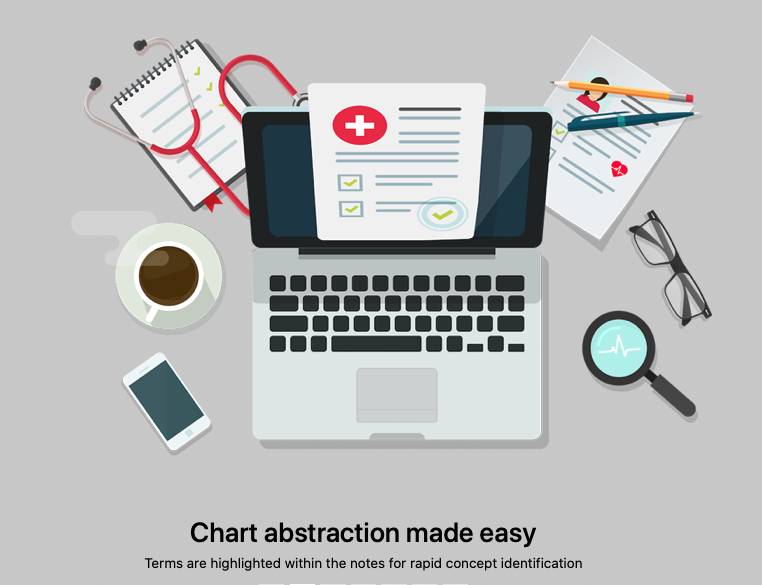
\includegraphics[width=0.8\linewidth]{Resources/Images/Banner1.png}
    \caption{An example figure for an opening graphic}
    \label{fig:emerse_banner1}
\end{figure}

This chapter is your introduction. Depending on your writing style, field of work, and project, you may choose to combine this into one chapter with the \texttt{\textbf{"Background"}} chapter.

This chapter is incorporated into the main body of writing by entering the following line(s) of command(s) in \texttt{thesis.tex}
\begin{verbatim}
# this line goes in the file "thesis.tex"
\chapter{Introduction}

%%%%%%%%%%%%%%%%%%%%%%%%%%%%%%%%%%%%%%%%%%%%%%%%%%%%%%%%%%%%%%%%%%%%%%%%%
%%%%%%%%%%%%%%%%%%%%% SECTION NAME %%%%%%%%%%%%%%%%%%%%%%%%%%%%%%%%%%%%%%
%%%%%%%%%%%%%%%%%%%%%%%%%%%%%%%%%%%%%%%%%%%%%%%%%%%%%%%%%%%%%%%%%%%%%%%%%
\section{SECTION NAME}
\begin{figure}
    \centering
    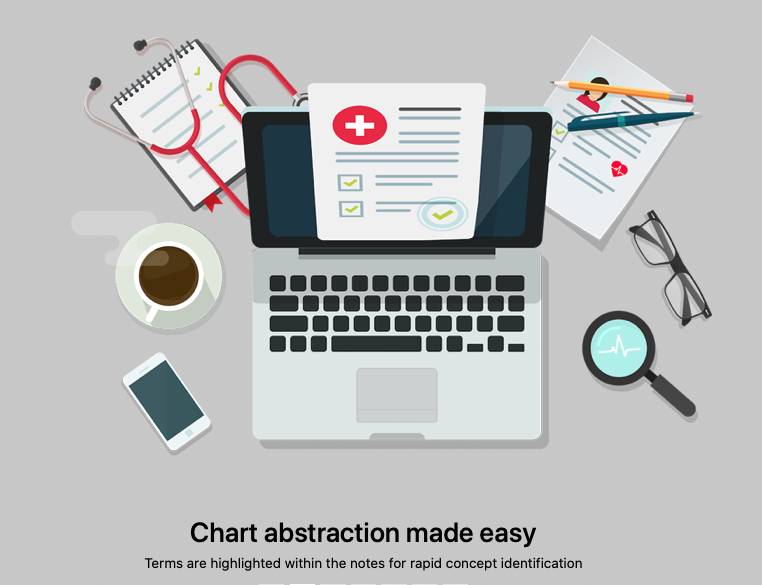
\includegraphics[width=0.8\linewidth]{Resources/Images/Banner1.png}
    \caption{An example figure for an opening graphic}
    \label{fig:emerse_banner1}
\end{figure}

This chapter is your introduction. Depending on your writing style, field of work, and project, you may choose to combine this into one chapter with the \texttt{\textbf{"Background"}} chapter.

This chapter is incorporated into the main body of writing by entering the following line(s) of command(s) in \texttt{thesis.tex}
\begin{verbatim}
# this line goes in the file "thesis.tex"
\chapter{Introduction}

%%%%%%%%%%%%%%%%%%%%%%%%%%%%%%%%%%%%%%%%%%%%%%%%%%%%%%%%%%%%%%%%%%%%%%%%%
%%%%%%%%%%%%%%%%%%%%% SECTION NAME %%%%%%%%%%%%%%%%%%%%%%%%%%%%%%%%%%%%%%
%%%%%%%%%%%%%%%%%%%%%%%%%%%%%%%%%%%%%%%%%%%%%%%%%%%%%%%%%%%%%%%%%%%%%%%%%
\section{SECTION NAME}
\begin{figure}
    \centering
    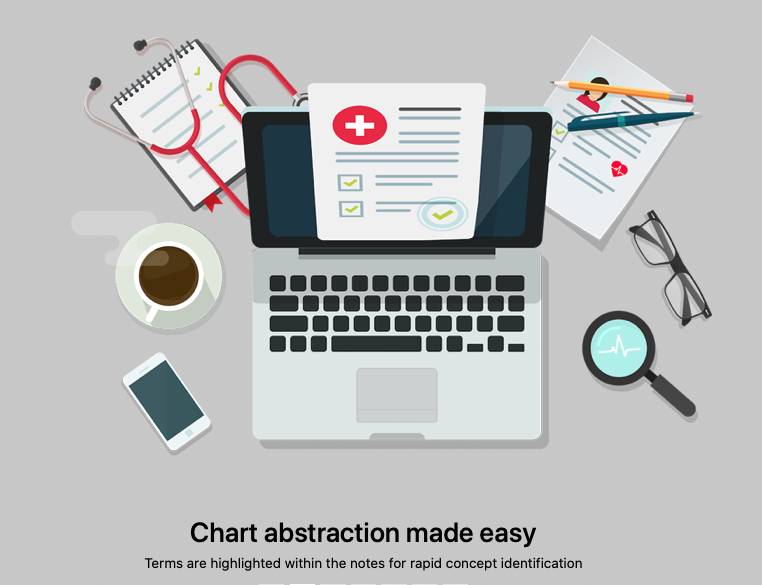
\includegraphics[width=0.8\linewidth]{Resources/Images/Banner1.png}
    \caption{An example figure for an opening graphic}
    \label{fig:emerse_banner1}
\end{figure}

This chapter is your introduction. Depending on your writing style, field of work, and project, you may choose to combine this into one chapter with the \texttt{\textbf{"Background"}} chapter.

This chapter is incorporated into the main body of writing by entering the following line(s) of command(s) in \texttt{thesis.tex}
\begin{verbatim}
# this line goes in the file "thesis.tex"
\chapter{Introduction}

%%%%%%%%%%%%%%%%%%%%%%%%%%%%%%%%%%%%%%%%%%%%%%%%%%%%%%%%%%%%%%%%%%%%%%%%%
%%%%%%%%%%%%%%%%%%%%% SECTION NAME %%%%%%%%%%%%%%%%%%%%%%%%%%%%%%%%%%%%%%
%%%%%%%%%%%%%%%%%%%%%%%%%%%%%%%%%%%%%%%%%%%%%%%%%%%%%%%%%%%%%%%%%%%%%%%%%
\section{SECTION NAME}
\begin{figure}
    \centering
    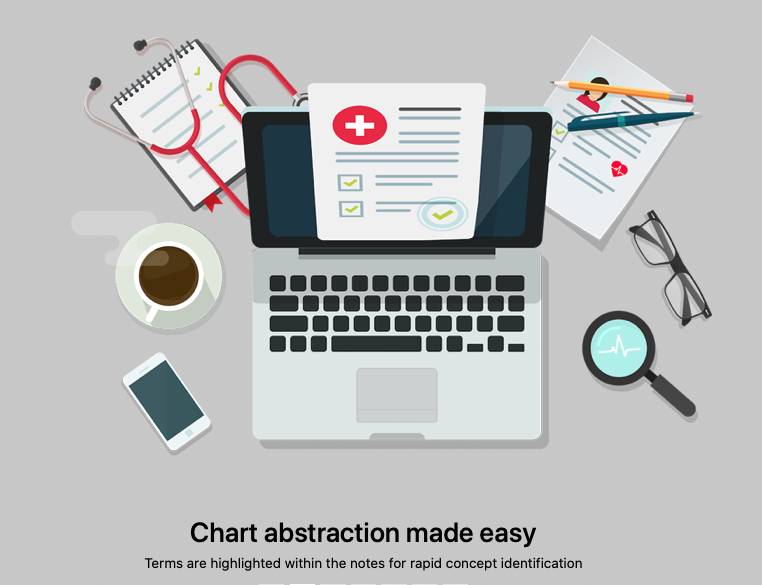
\includegraphics[width=0.8\linewidth]{Resources/Images/Banner1.png}
    \caption{An example figure for an opening graphic}
    \label{fig:emerse_banner1}
\end{figure}

This chapter is your introduction. Depending on your writing style, field of work, and project, you may choose to combine this into one chapter with the \texttt{\textbf{"Background"}} chapter.

This chapter is incorporated into the main body of writing by entering the following line(s) of command(s) in \texttt{thesis.tex}
\begin{verbatim}
# this line goes in the file "thesis.tex"
\include{Chapters/chapter1}
\end{verbatim}



%%% Local Variables: ***
%%% mode: latex ***
%%% TeX-master: "thesis.tex" ***
%%% End: ***

\end{verbatim}



%%% Local Variables: ***
%%% mode: latex ***
%%% TeX-master: "thesis.tex" ***
%%% End: ***

\end{verbatim}



%%% Local Variables: ***
%%% mode: latex ***
%%% TeX-master: "thesis.tex" ***
%%% End: ***

\end{verbatim}



%%% Local Variables: ***
%%% mode: latex ***
%%% TeX-master: "thesis.tex" ***
%%% End: ***
